%--------------------------------------------------------------------------------
% CONFIGURATION DU DOCUMENT
%--------------------------------------------------------------------------------

\documentclass[a4paper,12pt]{report}

\usepackage[french]{babel}
\usepackage[utf8]{inputenc}
\usepackage[T1]{fontenc}
\usepackage{mathptmx}
\usepackage[most]{tcolorbox}
\usepackage[a4paper, left=2.5cm, right=2.5cm, top=2.5cm, bottom=2.5cm]{geometry}
\usepackage{graphicx}
\usepackage{lipsum}
\usepackage{hyperref}
\usepackage{amsmath, amssymb}
\usepackage{array}
\usepackage{float}
\usepackage{tabularx}

\usepackage{pgfplots}
\usepackage{tikz} 
\usetikzlibrary{shapes.geometric, arrows, arrows.meta}

\pgfplotsset{
    /pgfplots/layers/Bowpark/.define layer set={
        axis background,axis grid,main,axis ticks,axis lines,axis tick labels,
        axis descriptions,axis foreground
    }{/pgfplots/layers/standard},
}


\setlength{\textfloatsep}{10pt}

\newcolumntype{Y}{>{\centering\arraybackslash}X}



\begin{document}





%--------------------------------------------------------------------------------
% PAGE DE GARDE
%--------------------------------------------------------------------------------

\begin{titlepage}
    \centering

    %----------------------------------
    % Informations sur l'université
    %----------------------------------

    {\large Faculté des Sciences et Ingénierie - Sorbonne Université}\\[0.3cm]
    {\large Master Informatique parcours ANDROIDE}\\[1cm]
    
\includegraphics[width=0.3\textwidth]{./images/logo_SU.png}\\[1.5cm]


    %----------------------------------
    % Informations sur le projet
    %----------------------------------

    \vspace{1.5cm}

    {\LARGE LRC - Logique et représentations des connaissances}\\[1cm]
    {\Large Rapport de projet}\\[2cm]
    \rule{\linewidth}{0.5mm} \\[1cm]
    {\Huge \textbf{Subsomptions en Prolog}} \\[0.4cm]
    \rule{\linewidth}{0.5mm} \\[2cm]
    

    %----------------------------------
    % Informations sur nous
    %----------------------------------

    \begin{flushleft}
        \textbf{Réalisé par :} \\[0.3cm]
        PINHO FERNANDES Enzo \\[0.2cm]
    \end{flushleft}
    

    %----------------------------------
    % Date
    %----------------------------------

    \vfill
    {\large Décembre 2024}\\
    
\end{titlepage}





%--------------------------------------------------------------------------------
% Table des matières
%--------------------------------------------------------------------------------

\tableofcontents





%--------------------------------------------------------------------------------
% Pages d'introduction
%--------------------------------------------------------------------------------

\newpage

\chapter*{Introduction}
\addcontentsline{toc}{chapter}{Introduction}

Le but de ce projet est de programmer en Prolog un algorithme permettant d'inférer des subsomptions pour la logique de description \(FL^-\) décrite à la fin du sujet.
    On procède de façon progressive en ajoutant des règles pour gérer des cas de plus en plus complexes. On s'assure toujours de faire des inférences correctes : si on trouve
    que \(C\) subsume \(D\) selon nos règles, on a la garantie que \(C\) subsume bien \(D\). L'inverse n'est pas forcément vrai, le programme, construit progressivement, pouvant
    être incomplet.\\

Le rendu du projet doit comporter deux fichiers :
\begin{itemize}
    \item un fichier prolog, comportant en première ligne, en commentaire, les prénoms et noms des deux membres du binôme,
    \item un fichier pdf, comportant également en première ligne les prénoms et noms des deux membres du binôme et donnant les réponses aux questions de commentaire et logique.
\end{itemize}

\newpage





%--------------------------------------------------------------------------------
% Représentation
%--------------------------------------------------------------------------------

\newpage

\chapter*{Représentation}
\addcontentsline{toc}{chapter}{Représentation}





%--------------------------------------------------------------------------------
% Exercice 1
%--------------------------------------------------------------------------------

\section*{Exercice 1 : Représentation préfixe en prolog}
\addcontentsline{toc}{section}{Représentation préfixe en prolog}

On traduit les différents opérateurs de concepts et éléments des T-Box et A-Box de la façon suivante :
\begin{center}
    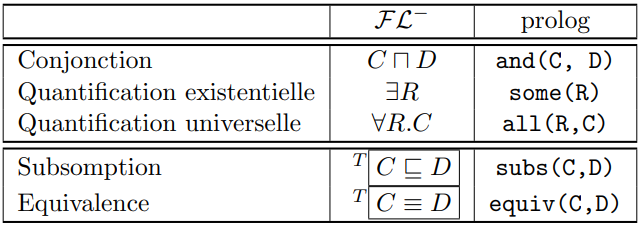
\includegraphics[width=0.6\textwidth]{./images/traduction_op.png}\\[1.5cm]
\end{center}

On travaille sur la T-Box correspondant aux connaissances sur les animaux suivant :
\begin{center}
    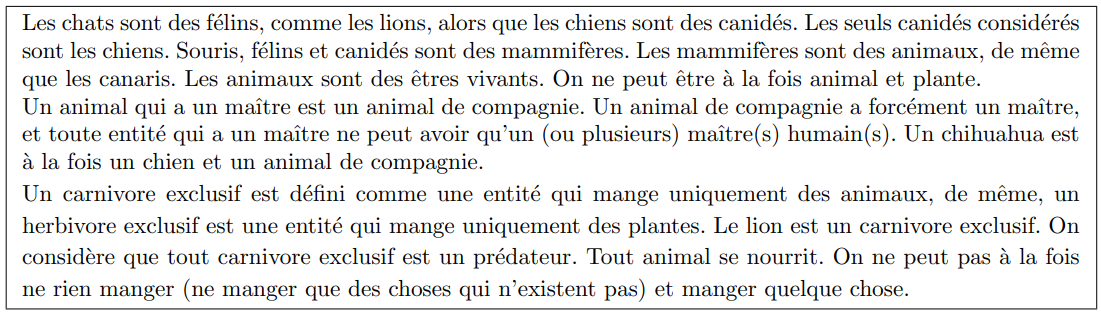
\includegraphics[width=1\textwidth]{./images/description_animaux.png}\\[1.5cm]
\end{center}

La traduction de ces connaissances en prolog est donnée dans le fichier \href{./src/LRC\_donneesProjet.pl}{LRC\_donneesProjet.pl}.
    Ouvrir ce fichier pour inspecter les données. Traduire en formules de \(FL^-\) les 6 lignes associées à l'indication \textbf{/* à commenter */} et
    identifier les phrases qu'elles traduisent.\\
    Note : \(\bot\) n'existant pas en \(FL^-\), on traite ici \textbf{nothing} comme un concept atomique.



\newpage

\begin{tcolorbox}[colback=gray!10, colframe=blue!30, coltitle=black, title=Réponse à l'exercice 1 - 1/1]

    Voici la traduction en \(FL^-\) des 6 lignes à commenter du fichier \href{./src/LRC\_donneesProjet.pl}{LRC\_donneesProjet.pl} ainsi que l'identification
        des phrases qu'elles traduisent dans la description des animaux vu précédemment.

    \begin{table}[H]
        \centering
        \setlength{\tabcolsep}{10pt}
        \begin{tabularx}{\textwidth}{|Y|}

            \hline \\[-0.4cm]
            \textbf{Code prolog} \\[0.3cm]
            \textbf{Traduction \(FL^-\)} \\[0.3cm]
            \textbf{Identification de la phrase} \\[0.1cm]
            \hline

            \hline \\[-0.4cm]
            \texttt{subs(chat,felin).} \\[0.3cm]
            \(chat \sqsubseteq felin\) \\[0.3cm]
            "Les chats sont des félins" \\[0.1cm]
            \hline

            \hline \\[-0.4cm]
            \texttt{subs(chihuahua,and(chien,pet)).} \\[0.3cm]
            \(chihuahua \sqsubseteq (chien \sqcap pet) \) \\[0.3cm]
            "Un chihuahua est à la fois un chien et un animal de compagnie." \\[0.1cm]
            \hline

            \hline \\[-0.4cm]
            \texttt{subs(and(animal,some(aMaitre)),pet).} \\[0.3cm]
            \((animal \sqcap \exists aMaitre) \sqsubseteq pet\) \\[0.3cm]
            "Un animal qui a un maître est un animal de compagnie." \\[0.1cm]
            \hline

            \hline \\[-0.4cm]
            \texttt{subs(some(aMaitre),all(aMaitre,personne)).} \\[0.3cm]
            \(\exists aMaitre \sqsubseteq \forall aMaitre.personne\) \\[0.3cm]
            "Toute entité qui a un maître ne peut avoir qu'un (ou plusieurs) maître(s) humain(s)." \\[0.1cm]
            \hline

            \hline \\[-0.4cm]
            \texttt{subs(and(all(mange,nothing),some(mange)),nothing).} \\[0.3cm]
            \((\forall mange.nothing \sqcap \exists mange) \sqsubseteq nothing\) \\[0.3cm]
            "On ne peut pas à la fois ne rien manger (ne manger que des choses qui n'existent pas) et manger quelque chose." \\[0.1cm]
            \hline

            \hline \\[-0.4cm]
            \texttt{equiv(carnivoreExc,all(mange,animal)).} \\[0.3cm]
            \(carnivoreExc \equiv \forall mange.animal\) \\[0.3cm]
            "Un carnivore exclusif est défini comme une entité qui mange uniquement des animaux." \\[0.1cm]
            \hline
            
        \end{tabularx}
    \end{table}

\end{tcolorbox}





%--------------------------------------------------------------------------------
% Subsomption structurelle pour FL-
%--------------------------------------------------------------------------------

\newpage

\chapter*{Subsomption structurelle pour \(FL^-\)}
\addcontentsline{toc}{chapter}{Subsomption structurelle pour \(FL^-\)}

Le but de cette section est d'écrire un ensemble de règles permettant de répondre à des questions du type "est-ce qu'on peut prouver que \(C\) est
    subsumé par \(D\) ?" (soit "est-ce que \(C \sqsubseteq_s D ?\)")\\

Il faut souligner la différentre entre \(\sqsubseteq\), qui correspond à des axiomes d'inclusion fournis explicitement dans la TBox, et \(\sqsubseteq_s\),
    qui correspond à des subsomptions que l'on peut prouver, à partir des axiomes fournis dans la TBox.





%--------------------------------------------------------------------------------
% Exercice 2
%--------------------------------------------------------------------------------

\section*{Exercice 2 : Concepts atomiques}
\addcontentsline{toc}{section}{Concepts atomiques}

On suppose que dans un premier temps que la TBox ne contient que des expressions du type \(A \sqsubseteq B\) où \(A\) et \(B\) sont des concepts
    atomiques et que \(C\) et \(D\) sont aussi atomiques. Pour vérifier si \(C \sqsubseteq_s D\) dans ce contexte, on propose les règles suivantes,
    à écrire dans votre fichier prolog, dans lequel vous aurez préalablement copié-collé le contenu du fichier \href{./src/LRC\_donneesProjet.pl}{LRC\_donneesProjet.pl}.\\\\
\texttt{subsS1(C,C).}\\
\texttt{subsS1(C,D) : -subs(C,D), C\textbackslash==D.}\\
\texttt{subsS1(C,D) : -subs(C,E), subsS1(E,D).}\\



%--------------------------------------------------------------------------------
% Question 2.1
%--------------------------------------------------------------------------------

\vspace{0.5cm}

\phantomsection
\addcontentsline{toc}{subsection}{1. Traduction des règles et tests}

\textbf{2.1)} Que traduisent ces règles ? Les tester sur les requêtes \(canari \sqsubseteq_s animal\), \(chat \sqsubseteq_s etreVivant\).



\begin{tcolorbox}[colback=gray!10, colframe=blue!30, coltitle=black, title=Réponse à la question 2.1 - 1/1]

    \textbf{Traduction des règles :}\\[-0.4cm]
    \begin{itemize}
        \item \texttt{subsS1(C,C)} : 
        \begin{itemize}
            \item Un concept est toujours subsumé par lui-même, on a donc \(C \sqsubseteq_s C\).
        \end{itemize}
        \vspace{0.3cm}

        \item \texttt{subsS1(C,D) :- subs(C,D), C\textbackslash==D} : 
        \begin{itemize}
            \item Si, dans la TBox, un concept \(C\) est subsumé par un concept \(D\) différent, alors on a \(C \sqsubseteq_s D\).
        \end{itemize}
        \vspace{0.3cm}

        \item \texttt{subsS1(C,D) :- subs(C,E), subsS1(E,D)} : 
        \begin{itemize}
            \item On peut y voir la règle de la transitivité. Si \(C \sqsubseteq E\), et \(E \sqsubseteq_s D\), alors on a \(C \sqsubseteq D\).
        \end{itemize}
    \end{itemize}

    \vspace{0.5cm}
    \hrule
    \vspace{0.5cm}

    Les requêtes renvoient true, ce qui est logique pour la première étant donné qu'on a bien \(canari \sqsubseteq animal\). Pour la deuxième, il existe une transition
        qui part de \(chat\) et qui arrive à \(etreVivant\), la voici : \((chat \sqsubseteq felin) \rightarrow (felin \sqsubseteq mammifere) \rightarrow (mammifere \sqsubseteq animal) 
        \rightarrow (animal \sqsubseteq etreVivant)\).  

\end{tcolorbox}



%--------------------------------------------------------------------------------
% Question 2.2
%--------------------------------------------------------------------------------

\newpage

\phantomsection
\addcontentsline{toc}{subsection}{2. Problème de la requête \(chien \sqsubseteq_s  souris\)}

\textbf{2.2)} Tester la requête \(chien \sqsubseteq_s  souris\). Quel problème pose cette requête ? Utiliser la trace pour en identifier la cause.



\begin{tcolorbox}[colback=gray!10, colframe=blue!30, coltitle=black, title=Réponse à la question 2.2 - 1/1]

    La requête \(chien \sqsubseteq_s  souris\) ne se termine jamais, dû à une boucle infinie au niveau de la règle de la transition. En effet, étant
        donné que \(chien\) et \(souris\) ne sont pas les mêmes concepts, et que nous avons pas \(chien \sqsubseteq souris\), alors le seul moyen est
        de trouver une transition de subsomption possible entre les deux.\\

    Pour cela, il essayera de commencer par la subsomption \(chien \sqsubseteq canide\) et cherchera donc à vérifier \(canide \sqsubseteq souris\). Même
        constat pour celui-ci. Il essayera plusieurs transitions qui rateront, jusqu'à qu'il fasse une transition \(canide \sqsubseteq chien\)... Et il
        cherchera à vérifier la requête initiale \(chien \sqsubseteq_s  souris\). Cela crée une boucle infinie.

    \vspace{0.5cm}
    \hrule
    \vspace{0.5cm}

    Voici l'exécution de la requête avec trace, et quelques commentaires dessus pointant le problème.
    \begin{center}
        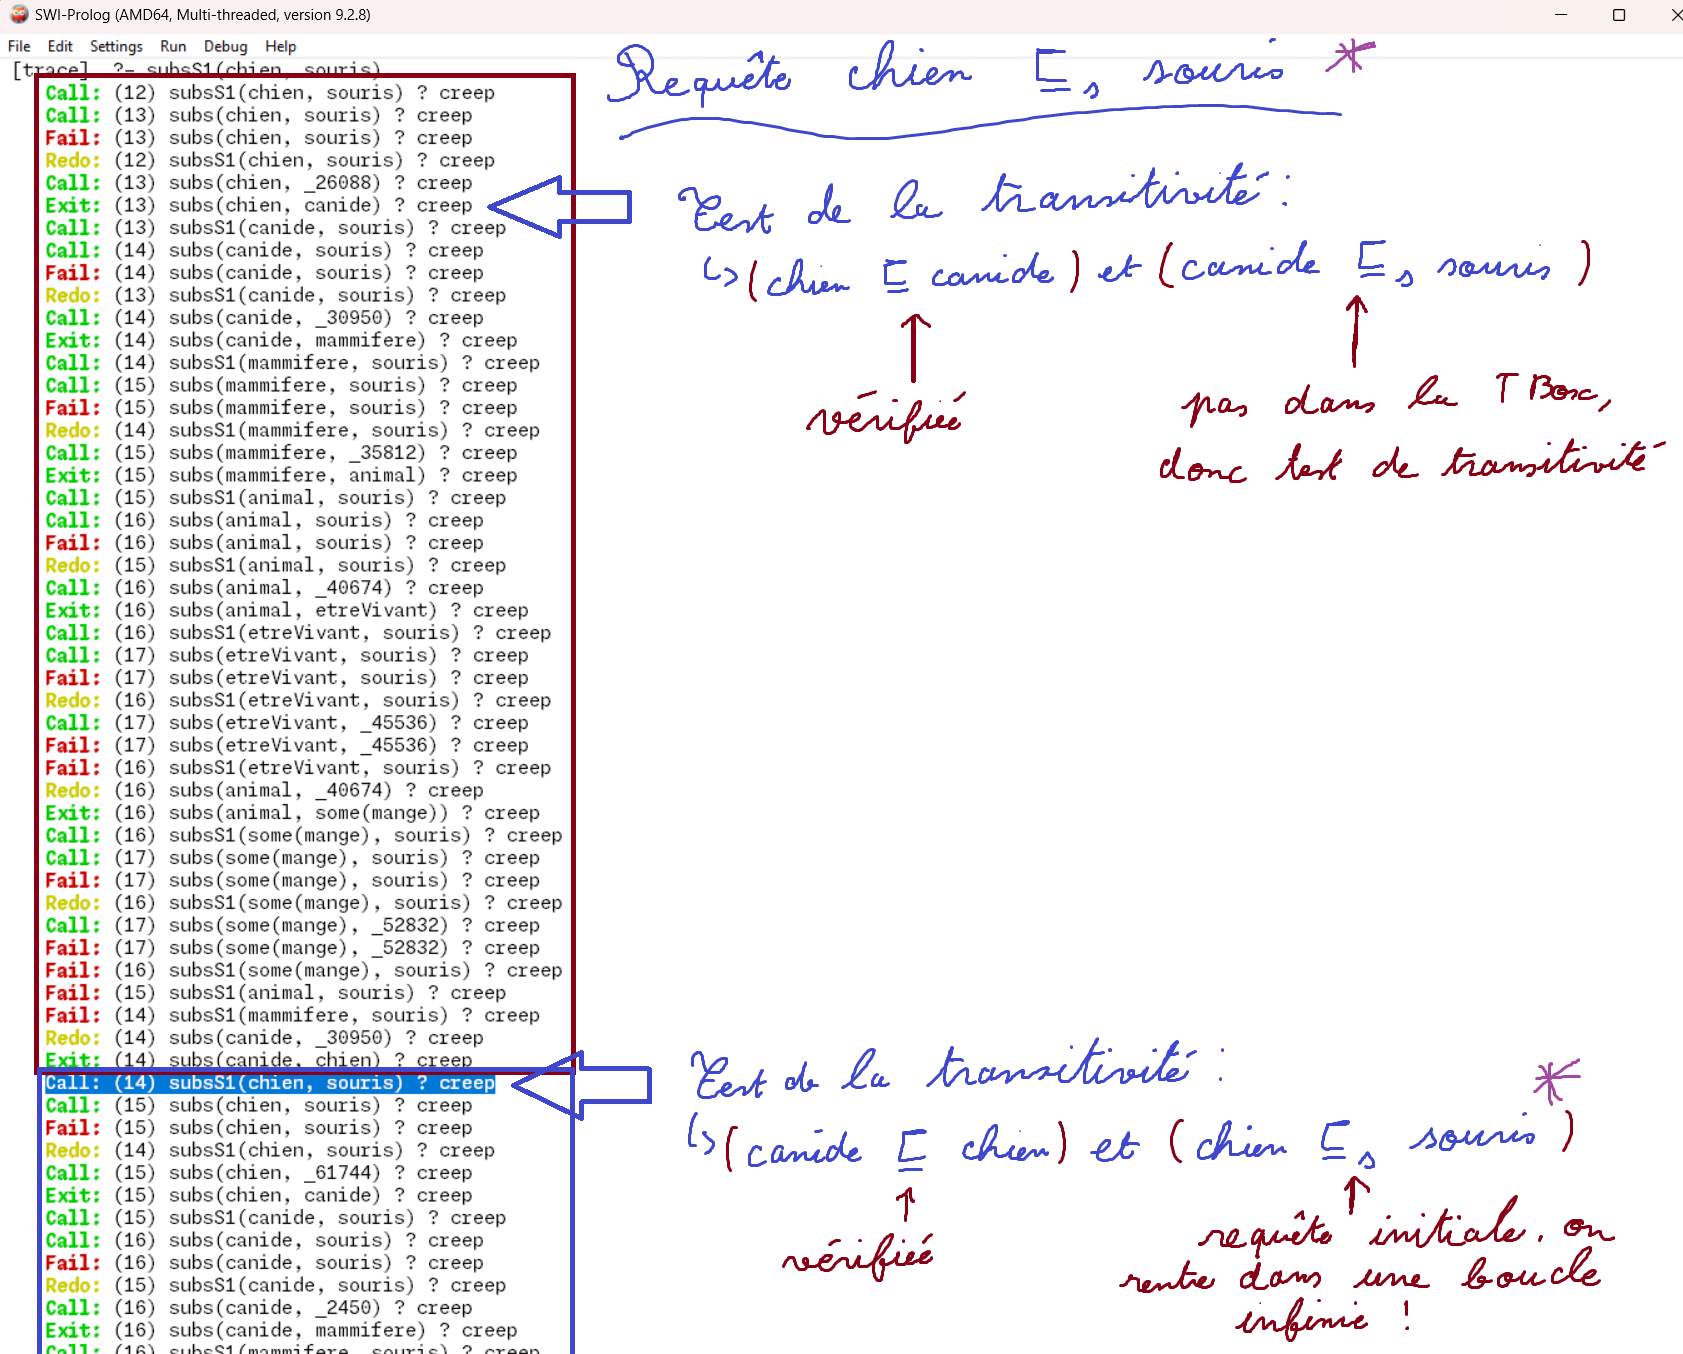
\includegraphics[width=1\textwidth]{./images/chien_souris_infini.png}\\[1.5cm]
    \end{center}


\end{tcolorbox}



%--------------------------------------------------------------------------------
% Question 2.3
%--------------------------------------------------------------------------------

\newpage

Pour corriger ce problème, on introduit un troisième argument contenant la liste des subsomptions déjà faites dans une branche. On définit \texttt{subsS(C,D)},
    qui doit être vérifié quand \(C \sqsubseteq_s D\), avec le prédicat auxiliaire \texttt{subsS(C,D,L)} où \(L\) contient la liste des concepts utilisés
    dans la preuve de la subsomption. Pour éviter des preuves infinies, on s'interdit de réutiliser un concept déjà présent dans \(L\).\\

On réécrit donc les règles sur \texttt{subsS1(C,D)} pour définir \texttt{subsS(C,D,L)}, en ajoutant avant tout appel récursif \(E \sqsubseteq_s D\)
    la condition que \(E\) ne soit pas dans \(L\) et en ajoutant \(E\) à \(L\) dans l'appel récursif :\\\\
\texttt{subsS(C,D) :- subsS(C,D,[C]).}\\
\texttt{subsS(C,C,\_).}\\
\texttt{subsS(C,D,\_) :- subs(C,D), C \textbackslash== D}\\
\texttt{subsS(C,D,L) : -subs(C,E), not(member(E,L)), subsS(E,D,[E|L]), E \textbackslash== D.}\\



\vspace{0.5cm}

\phantomsection
\addcontentsline{toc}{subsection}{3. Tests des nouvelles règles}



\textbf{2.3)} Tester ces nouvelles règles avec \(chat \sqsubseteq_s etreVivant\), \(chien \sqsubseteq_s canide\) et \(chien \sqsubseteq_s chien\) et
    vérifier que le résultat est conforme aux attentes. Tester ensuite la requête \(chien \sqsubseteq_s souris\) qui doit échouer. Inspecter la trace
    de cette requête.



\begin{tcolorbox}[colback=gray!10, colframe=blue!30, coltitle=black, title=Réponse à la question 2.3 - 1/1]

    Les requêtes \(chat \sqsubseteq_s etreVivant\), \(chien \sqsubseteq_s canide\) et \(chien \sqsubseteq_s chien\) renvoient tous true, ce qui est conforme
        à nos attentes. En ce qui concerne la requête \(chien \sqsubseteq_s souris\), elle échoue bien comme attendu. Avec la trace, nous pouvons constater
        qu'à chaque transition testée, on vérifie le contenu de la liste des concepts utilisés. Et celui-ci empêche bien la boucle infinie dû à la transition de
        \(canide\) et \(chien\).

    \vspace{0.5cm}
    \hrule
    \vspace{0.5cm}

    Voici l'exécution d'un bout de requête avec trace, sur la solution du problème de la boucle infinie.
    \begin{center}
        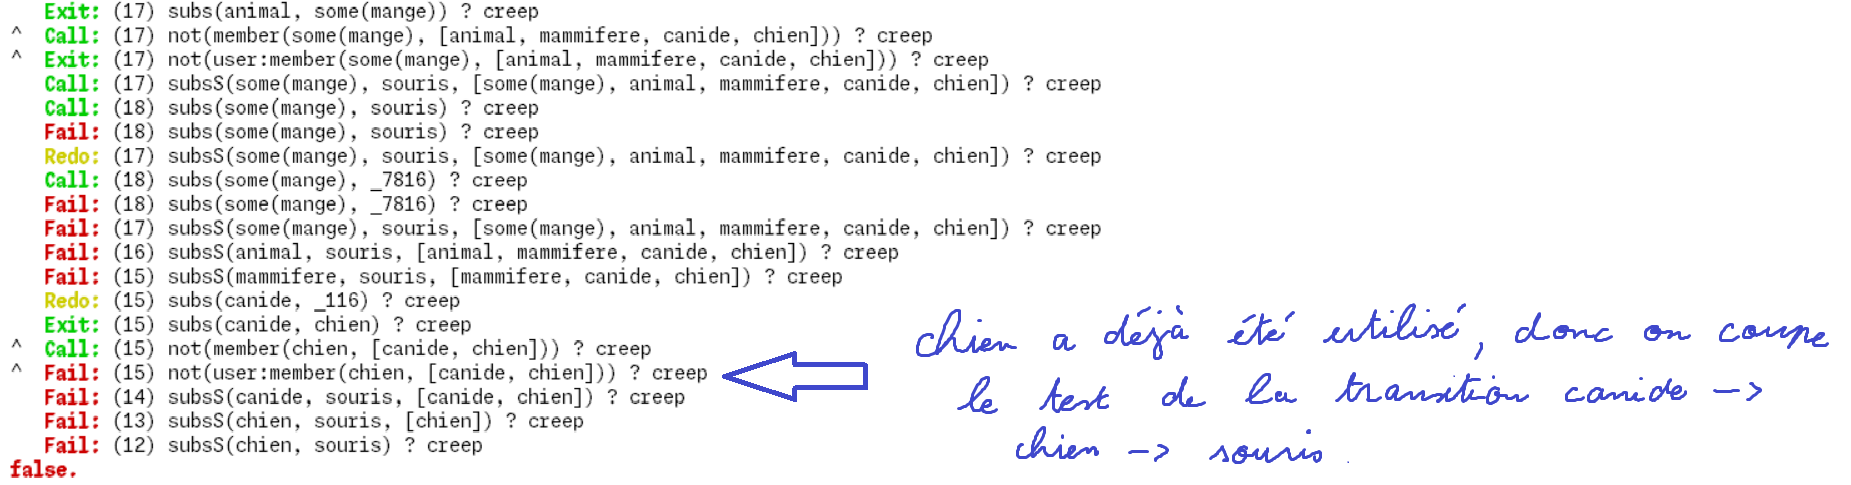
\includegraphics[width=1\textwidth]{./images/chien_souris_not_infini.png}\\[1.5cm]
    \end{center}

\end{tcolorbox}



%--------------------------------------------------------------------------------
% Question 2.4
%--------------------------------------------------------------------------------

\newpage

\phantomsection
\addcontentsline{toc}{subsection}{4. Test de la requête \(souris \sqsubseteq_s  \exists mange\)}

\textbf{2.4)} Tester la requête \(souris \sqsubseteq_s  \exists mange\). Pourquoi cette requête réussit-elle bien que \(\exists mange\) ne soit pas un concept atomique ?



\begin{tcolorbox}[colback=gray!10, colframe=blue!30, coltitle=black, title=Réponse à la question 2.4 - 1/1]

    Cette requête réussit bien que \(\exists mange\) n'est pas un concept atomique parce qu'il existe techniquement une transition de \(souris\) à \(some(mange)\)
        d'après notre TBox sur prolog. Ce dernier ne fait pas de "distinction" entre concept atomique et autre, et il trouve bien une valeur égale à \(some(mange)\).

    \vspace{0.5cm}
    \hrule
    \vspace{0.5cm}
        
    En effet, on peut suivre les étapes suivantes :\\[-0.4cm]
    \begin{itemize}
        \item \texttt{subsS(souris, some(mange)) :- subs(souris, mammifere), subsS(mammifere, some(mange))}\\[-0.2cm]
        \item \texttt{subs(souris, mammifere)} est vérifiée.
        \item \texttt{subsS(mammifere, some(mange)) :- subs(mammifere, animal), subsS(animal, some(mange))}\\[-0.2cm]
        \item \texttt{subs(mammifere, animal)} est vérifiée.
        \item \texttt{subsS(animal, some(mange))} est vérifiée grâce à la troisième règle, on trouve bien \texttt{subs(animal, some(mange))}.
    \end{itemize}

\end{tcolorbox}



%--------------------------------------------------------------------------------
% Question 2.5
%--------------------------------------------------------------------------------

\newpage

\phantomsection
\addcontentsline{toc}{subsection}{5. Requêtes \(chat \sqsubseteq_s X\) et \(X \sqsubseteq_s mammifere\)}

\textbf{2.5)} Que devraient renvoyer les requêtes \(chat \sqsubseteq_s X\) et \(X \sqsubseteq_s mammifere\) ? Vérifier que c'est bien le cas (il n'est pas nécessaire
    d'éliminer les réponses doubles ou le false final).



\begin{tcolorbox}[colback=gray!10, colframe=blue!30, coltitle=black, title=Réponse à la question 2.5 - 1/1]

    La requête \(chat \sqsubseteq_s X\) est sensée renvoyer "tout ce qu'un chat puisse être" par la variable X d'après notre TBox. Dans ce cas là, nous devrions avoir plusieurs
        résultats pour X. Un chat est un \textbf{chat} (subsumé par lui-même), un \textbf{félin}, un \textbf{mammifere}, un \textbf{animal}, un \textbf{être vivant} et
        pour la même raison qu'à la question 2.4, il devrait renvoyer \textbf{some(mange)}, parce qu'un animal mange toujours au moins une chose et que prolog le renvoie.\\

    \vspace{0.5cm}
    \hrule
    \vspace{0.5cm}
          
    La requête \(X \sqsubseteq_s mammifere\) est sensée renvoyer "toute entité étant un mammifere", dans notre TBox, les \textbf{félins, canidés et souris} seront renvoyés, ainsi 
        que \textbf{mammifère} parce que tout concept est subsumé par lui-même. Bien évidemment, on aura aussi les \textbf{chiens, chats et lions} qui seront renvoyés, parce qu'ils
        sont subsumés par \texttt{felin} et \texttt{canide}.

    \vspace{0.5cm}
    \hrule
    \vspace{0.5cm}

    Voici la vérification de notre réponse sur prolog, on a bien les mêmes résultats, ainsi qu'un false final, parce que Prolog teste d'autres possibilités même après avoir trouvé
        toutes les solutions réalisables.\\[0.5cm]
    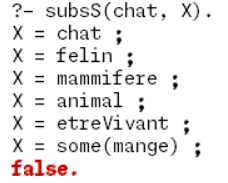
\includegraphics[width=0.5\textwidth]{./images/chat_X.png}
    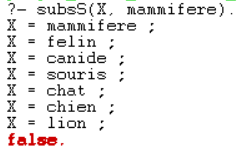
\includegraphics[width=0.5\textwidth]{./images/X_mammifere.png}

\end{tcolorbox}



%--------------------------------------------------------------------------------
% Question 2.6
%--------------------------------------------------------------------------------

\newpage

\phantomsection
\addcontentsline{toc}{subsection}{5. Règles pour l'équivalence, et requête \(lion \sqsubseteq_s \forall mange.animal\)}

\textbf{2.6)} Ecrire des règles permettant de dériver \(A \sqsubseteq B\) et \(B \sqsubseteq A\) à partir de \(A \equiv B\). Tester avant et 
    après ajout des règles la requête \(lion \sqsubseteq_s \forall mange.animal\).



\begin{tcolorbox}[colback=gray!10, colframe=blue!30, coltitle=black, title=Réponse à la question 2.6 - 1/1]

    Pour commencer, testons la requête avant l'ajout des règles. Prolog nous renvoie tout simplement \textbf{false}. En effet, nous avons aucune
        subsomption dans la TBox de type \(subs(X, all(mange, animal))\), \(X\) étant une variable. On ne peut donc pas trouver de transition, et 
        on ne peut pas utiliser l'équivalence \(carnivoreExc \equiv \forall mange.animal\) dû à l'absence des règles.

    \vspace{0.5cm}
    \hrule
    \vspace{0.5cm}

    Afin d'ajouter les règles, il faut savoir que \(C \equiv D \Rightarrow (C \sqsubseteq D) \land (D \sqsubseteq C)\). Il suffit donc d'ajouter
        deux nouvelles règles cherchant si \(C \equiv D\) est dans la TBox, pour \(C \sqsubseteq D\) et \(D \sqsubseteq C\) séparémment. On a donc :\\\\
    \texttt{subs(C, D) :- equiv(C, D).}\\
    \texttt{subs(D, C) :- equiv(C, D).}\\

    L'ajout se trouve aux lignes 61-63 du fichier \href{./src/LRC\_donneesProjet.pl}{LRC\_donneesProjet.pl}.

    \vspace{0.5cm}
    \hrule
    \vspace{0.5cm}

    Avec les nouvelles règles, prolog nous renvoie \textbf{true}. En effet, il va en premier lieu tester plusieurs transitions de subsomption jusqu'à tomber
        sur celle allant de \(lion\) à \(carnivoreExc\). Ensuite, il essayera donc de prouver que \(subsS(carnivoreExc, all(mange, animal))\) ce qu'il y arrivera
        grâce à l'équivalence \(equiv(carnivoreExc, all(mange, animal))\).\\

    Ensuite, il cherchera toujours d'autres chemins possible, sans résultat, renvoyant un false.

\end{tcolorbox}





%--------------------------------------------------------------------------------
% Exercice 3
%--------------------------------------------------------------------------------

\newpage
\section*{Exercice 3 : Gestion des conjonctions}
\addcontentsline{toc}{section}{Gestion des conjonctions}

On s'intéresse maintenant aux requêtes contenant des conjonctions de concepts. On étend donc la définition du prédicat \texttt{subsS} avec les règles données dans le 
    fichier \href{./src/LRC\_donneesProjet.pl}{LRC\_donneesProjet.pl}. Il est important de travailler dans le même fichier et de garder le même nom de prédicat (\texttt{subsS})
    afin que la définition soit étendue et non remplacée. Il faut donc recopier les règles du fichier \href{./src/LRC\_reglesConjonction.pl}{LRC\_reglesConjonction.pl}
    dans votre fichier prolog, à la suite des règles écrites pour l'exercice précédent.



%--------------------------------------------------------------------------------
% Question 3.1
%--------------------------------------------------------------------------------

\vspace{0.5cm}

\phantomsection
\addcontentsline{toc}{subsection}{1. Tests de requêtes}

\textbf{3.1)} Tester cet ensemble de règles avec les requêtes \(chihuahua \sqsubseteq_s (mammifere \sqcap \exists aMaitre)\), \((chien \sqcap \exists aMaitre) \sqsubseteq_s pet\)
    et \(chihuahua \sqsubseteq_s (pet \sqcap chien)\).



\begin{tcolorbox}[colback=gray!10, colframe=blue!30, coltitle=black, title=Réponse à la question 3.1 - 1/1]

    Les trois requêtes renvoient true avec ces nouvelles règles. 
    
    \vspace{0.5cm}
    \hrule
    \vspace{0.5cm}

    Sans ces dernières, prolog aurait considéré les conjonctions comme un concept atomique (comme pour le quantificateur \(\exists\)). Par conséquent, tant que la 
        requête n'est pas dans la TBox ou qu'il n'existe pas de transition pour arriver au résultat souhaité, il est impossible d'approuver la subsomption alors
        qu'elle existe.

\end{tcolorbox}



%--------------------------------------------------------------------------------
% Question 3.2
%--------------------------------------------------------------------------------

\newpage

\phantomsection
\addcontentsline{toc}{subsection}{2. Situation traitée par chaque règle}

\textbf{3.2)} Pour chacune des règles, indiquer la situation traitée par la règle et donner un exemple de requête qui échouerait sans la règle. Ces exemples peuvent
    utiliser la TBox donnée directement (pas forcément possible pour toutes les règles), la compléter pour illustrer une situation particulière, ou en proposer pour
    une nouvelle assez simple pour illustrer l'utilité de chaque règle.



\begin{tcolorbox}[colback=gray!10, colframe=blue!30, coltitle=black, title=Réponse à la question 3.2 - 1/2]

    \texttt{subsS(C, and(D1,D2), L) :- D1 \textbackslash= D2, subsS(C,D1,L), subsS(C,D2,L)} :\\[-0.4cm]
    \begin{itemize}
        \item \textbf{Situation :} Cette règle permet de vérifier si un concept \(C\) est subsumé par la conjonction de deux concepts \(D_1\) et \(D_2\).
        
        \vspace{0.1cm}
        \item \textbf{Exemple d'échec :} \texttt{subsS(canari, and(animal, etreVivant))}.
    \end{itemize}


    \vspace{0.5cm}
    \hrule
    \vspace{0.5cm}


    \texttt{subsS(C, D, L) :- subs(and(D1, D2), D), E = and(D1, D2), not(member(E, L)), subsS(C, E, [E|L]), E \textbackslash== C} :\\[-0.4cm]
    \begin{itemize}
        \item \textbf{Situation :} Cette règle permet de vérifier si un concept \(C\) est subsumé par un concept \(D\), ce dernier étant d'ailleurs subsumé par une 
            conjonction de concepts \(D_1\) et \(D_2\). On utilise donc une transition en passant par une conjonction.
        
        \vspace{0.1cm}
        \item \textbf{Exemple d'échec :} \texttt{subsS(canariPet, pet)}. Nous avons ajouté dans la TBox \texttt{subs(canariPet, canari)} et subs(canariPet, some(aMaitre))
            pour créer le cas où un canari spécifique est un animal de compagnie. En effet, il existe une transition grâce à \texttt{subs(and(animal,some(aMaitre)),pet)}.
            Sans cette règle, la requête renvoierait false.
    \end{itemize}
    

    \vspace{0.5cm}
    \hrule
    \vspace{0.5cm}


    \texttt{subsS(and(C, C), D, L) :- nonvar(C), subsS(C, D, [C|L])} :
    \begin{itemize}
        \item \textbf{Situation :} Cette règle permet de vérifier le cas d'une requête où on a une conjonction de deux concepts identiques (ici \(C\)). En effet, \(C \sqcap C\) 
            équivaut à \(C\), tout simplement.
        
        \vspace{0.1cm}
        \item \textbf{Exemple d'échec :} \texttt{subsS(and(canari, canari), animal)}.
    \end{itemize}


    \vspace{0.5cm}
    \hrule
    \vspace{0.5cm}


    \texttt{subsS(and(C1, C2), D, L) :- C1 \textbackslash= C2, subsS(C1, D, [C1|L])},\\
    \texttt{subsS(and(C1, C2), D, L) :- C1 \textbackslash= C2, subsS(C2, D, [C1|L])} :\\[-0.4cm]
    \begin{itemize}
        \item \textbf{Situation :} Ces deux règles permet de vérifier si une conjonction de deux concepts différents \(C_1\) et \(C_2\) est subsumé par un concept \(D\).
            Pour cela, elles vérifient si \(C_1\) ou \(C_2\) est subsumé par \(D\). Il suffit que l'un d'entre eux le soit pour que la requête renvoit une réponse positive.
        
        \vspace{0.1cm}
        \item \textbf{Exemple d'échec :} \texttt{subsS(and(chien, animal), mammifere)}.
    \end{itemize}

\end{tcolorbox}
\begin{tcolorbox}[colback=gray!10, colframe=blue!30, coltitle=black, title=Réponse à la question 3.2 - 2/2]

    \texttt{subsS(and(C1, C2), D, L) :- subs(C1, E1), E = and(E1, C2), not(member(E, L)), subsS(E, D, [E|L]), E \textbackslash== D} :\\[-0.4cm]
    \begin{itemize}
        \item \textbf{Situation :} Cette règle permet de vérifier la même chose que les deux règles précédentes, avec une autre méthode. Ici, on essaye de remplacer la
            première composante de la conjonction \((C_1)\) avec un concept \(E_1\) qui le subsume. Ainsi, si \texttt{subsS(and(E1, C2), D, L)} est vraie, alors la 
            requête initiale aussi.
        
        \vspace{0.1cm}
        \item \textbf{Exemple d'échec :} \texttt{subsS(and(canari, some(aMaitre)), pet)}. En effet, on a dans la TBox \texttt{subs(canari,animal)} et 
            \texttt{subs(and(animal,some(aMaitre)),pet)}. Avec cette règle, on a bien une requête réussite. Sinon, non. 
    \end{itemize}


    \vspace{0.5cm}
    \hrule
    \vspace{0.5cm}


    \texttt{subsS(and(C1, C2), D, L) :- subs(C1, E1), E = and(E1, C2), not(member(E, L)), subsS(E, D, [E|L]), E \textbackslash== D} :\\[-0.4cm]
    \begin{itemize}
        \item \textbf{Situation :} Cette règle permet de, si les autres règles n'ont pas suffit, d'inverser les deux composantes de la conjonction. En effet, 
            \(C_1 \sqcap C_2\) équivaut à \(C_2 \sqcap C_1\). On recommence la recherche avec l'inversion, en usant des règles précédentes.
        
        \vspace{0.1cm}
        \item \textbf{Exemple d'échec :} \texttt{subsS(and(homme, parent), pere)}. Nous avons ajouté dans la TBox \texttt{subs(and(parent, homme), pere)}. La requête
            émise inverse les deux composantes de la conjonction. Sans cette règle, prolog ne peut pas considéré ce cas là.
    \end{itemize}

\end{tcolorbox}





%--------------------------------------------------------------------------------
% Exercice 4
%--------------------------------------------------------------------------------

\newpage
\section*{Exercice 4 : Gestion des rôles}
\addcontentsline{toc}{section}{Gestion des rôles}

On s'intéresse maintenant aux requêtes contenant des rôles qualifiés, c'est-à-dire de la forme \(\forall R.C\).



%--------------------------------------------------------------------------------
% Question 4.1
%--------------------------------------------------------------------------------

\vspace{0.5cm}

\phantomsection
\addcontentsline{toc}{subsection}{1. Règle pour les requêtes type \(\forall R.C \sqsubseteq_s \forall R.D \)}

\textbf{4.1)} Ecrire une règle permettant de répondre à une requête du type \(\forall R.C \sqsubseteq_s \forall R.D \), où \(C\) et \(D\) sont des concepts à partir de
    \(C\) et \(D\). Il s'agit là encore d'étendre la définition de \texttt{subsS} et non de créer un nouveau prédicat.



\begin{tcolorbox}[colback=gray!10, colframe=blue!30, coltitle=black, title=Réponse à la question 4.1 - 1/1]

    Nous savons que \((C \sqsubseteq_s D) \Rightarrow (\forall R.C \sqsubseteq_s \forall R.D)\). Par conséquent, la règle à écrire est :
    \begin{center}
        \texttt{subsS(all(R, C), all(R, D), L) :- subsS(C, D, L).}
    \end{center}

\end{tcolorbox}



%--------------------------------------------------------------------------------
% Question 4.2
%--------------------------------------------------------------------------------

\vspace{0.5cm}

\phantomsection
\addcontentsline{toc}{subsection}{2. Tests de requêtes}

\textbf{4.2)} Tester les requêtes \(lion \sqsubseteq_s \forall mange.etreVivant\) et \(\forall mange.canari \sqsubseteq carnivoreExc\).



\begin{tcolorbox}[colback=gray!10, colframe=blue!30, coltitle=black, title=Réponse à la question 4.2 - 1/1]

    La requête \texttt{subsS(lion, all(mange, etreVivant))} renvoie true, étant le résultat logique.

    \vspace{0.5cm}
    \hrule
    \vspace{0.5cm}

    La requête \texttt{subsS(all(mange, canari), carnivoreExc)} renvoie false, ce qui n'est pas le résultat souhaité. Une entité qui ne mange que des canaris est une 
        entité qui ne mange que des animaux, donc un carnivore exclusive.

\end{tcolorbox}



%--------------------------------------------------------------------------------
% Question 4.3
%--------------------------------------------------------------------------------

\newpage

\phantomsection
\addcontentsline{toc}{subsection}{3. Tests de requêtes et ajouts}

\textbf{4.3)} Tester les requêtes \((carnivoreExc \sqcap herbivoreExc) \sqsubseteq_s \forall mange.nothing\) et 
    \(((carnivoreExc \sqcap herbivoreExc) \sqcap animal) \sqsubseteq_s nothing \).\\
    Si besoin, ajouter des règles pour qu'elles réussissent.\\
    Qu'en est-il de la requête \(((carnivoreExc \sqcap animal) \sqcap herbivoreExc) \sqsubseteq_s nothing\) ? Pourquoi ? (On n'exige pas de modifier le programme pour
    que cette dernière réussisse).



\begin{tcolorbox}[colback=gray!10, colframe=blue!30, coltitle=black, title=Réponse à la question 4.3 - 1/1]

    Initialement, les deux requêtes renvoient false. En effet, notre programme ne gère pas les contradictions/incohérences logiques (\texttt{nothing}) correctement.
        Par conséquent, pour que les deux requêtes renvoient true, nous avons ajouté les règles suivantes :\\\\
    \texttt{subsS(and(carnivoreExc, herbivoreExc), all(mange, nothing), L) :- not(member(nothing, L)).}\\\\
    \texttt{subsS(and(and(carnivoreExc, herbivoreExc), animal), nothing, L) :- not(member(nothing, L)).}


    \vspace{0.5cm}
    \hrule
    \vspace{0.5cm}

    La première règle permet de capturer l'incohérence entre \texttt{carnivoreExc} et \texttt{herbivoreExc}, et de la propager à \(\forall mange.nothing\).

    \vspace{0.5cm}
    \hrule
    \vspace{0.5cm}

    La seconde règle gère la situation où \texttt{carnivoreExc} et \texttt{herbivoreExc} est combinée à un autre concept extérieur, ici \texttt{animal}. Nous
        avons toujours une incohérence, bien qu'\texttt{animal} soit un concept valide.

    \vspace{0.5cm}
    \hrule
    \vspace{0.5cm}

    Enfin, la requête \texttt{subsS(and(and(carnivoreExc, animal), herbivoreExc), nothing)} échoue car on ne gère pas l'incohérence entre \texttt{carnivoreExc} et 
        \texttt{herbivoreExc} quand elles sont en conjonction avec un concept extérieur, ici \texttt{animal}. Il nous manque une règle générale pour gérer ces situations,
        qui permettrait de détecter les incohérences et ainsi les traiter afin d'avoir le résultat voulu/logique.

\end{tcolorbox}



%--------------------------------------------------------------------------------
% Question 4.4
%--------------------------------------------------------------------------------

\vspace{0.5cm}

\phantomsection
\addcontentsline{toc}{subsection}{4. Des règles similaires pour les concepts de la forme \(\exists R\) ?}

\textbf{4.4)} Est-il nécessaire d'écrire des règles similaires pour les concepts de la forme \(\exists R\) ?



\begin{tcolorbox}[colback=gray!10, colframe=blue!30, coltitle=black, title=Réponse à la question 4.4 - 1/1]

    \textbf{Non}, il n'est pas nécessaire d'écrire des règles similaires pour les concepts de la forme \(\exists R\). Comme dit précédemment à la question 2.4,
        notre programme couvre déjà les quantifications existencielles parce qu'elles sont exprimées "comme des concepts atomiques". Chaque règle marche correctement
        avec ce cas là.


\end{tcolorbox}



%--------------------------------------------------------------------------------
% Question 4.5
%--------------------------------------------------------------------------------

\newpage

\phantomsection
\addcontentsline{toc}{subsection}{5. Les requêtes \(lion \sqsubseteq_s X\) et \(X \sqsubseteq_s predateur\) ?}

\textbf{4.5)} Que devraient renvoyer les requêtes \(lion \sqsubseteq_s X\) et \(X \sqsubseteq_s predateur\) ? Voir si c'est bien le cas avec vos règles
    (il n'est pas nécessaire d'éliminer les réponses doubles ou le false final).



\begin{tcolorbox}[colback=gray!10, colframe=blue!30, coltitle=black, title=Réponse à la question 4.5 - 1/1]

    Pour la requête \texttt{subsS(lion, X)}, on doit avoir "tout ce qu'est un lion". Logiquement, d'après notre TBox, un lion est un \textbf{lion} (subsumé par lui-même),
        un \textbf{félin}, un \textbf{carnivoreExc} ,un \textbf{mammifere}, un \textbf{animal}, un \textbf{être vivant}, et \textbf{some(mange)} pour la même justification qu'avec 
        \(chat \sqsubseteq_s X\) à la question 2.5.\\
    
    Mais maintenant, nous avons implémenté des règles pour la gestion des rôles ! Logiquement, prolog devrait renvoyer les rôles du lion. Ce sera à propos de son alimentation.
        Il ne mange que des animaux (\textbf{all(mange, animal)}), et des êtres vivants (\textbf{all(mange, etreVivant)}) étant donné qu'\texttt{animal} est subsumé par 
        \texttt{etreVivant}. Et enfin, pour la même justification, étant donné qu'on a \texttt{subs(animal,some(mange))}, prolog doit renvoyer \textbf{all(mange, some(mange))}.

    
    \vspace{0.5cm}
    \hrule
    \vspace{0.5cm}


    Pour la requête \texttt{subsS(X, predateur)}, on doit avoir "toute entité étant un prédateur". Pour les mêmes raisons que précédemment en plus de la 2.5, on aurait donc un 
        \textbf{prédateur}, un \textbf{carnivoreExc}, un \textbf{lion} et toutes les conjonctions et rôles qui en découlent.


    \vspace{0.5cm}
    \hrule
    \vspace{0.5cm}


    Voici la vérification de notre réponse sur prolog, on a bien les mêmes résultats, ainsi qu'un false final.\\[0.5cm]
    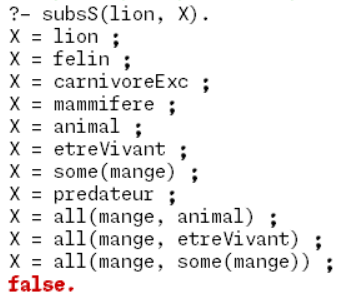
\includegraphics[width=0.41\textwidth]{./images/lion_X.png}
    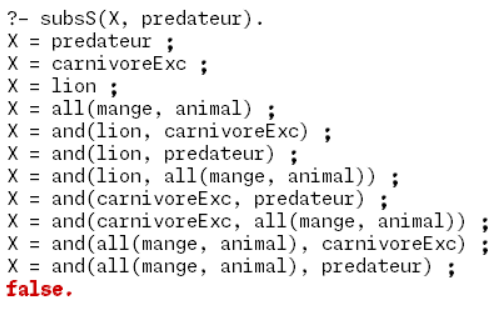
\includegraphics[width=0.59\textwidth]{./images/X_predateur.png}

\end{tcolorbox}





%--------------------------------------------------------------------------------
% Exercice 5
%--------------------------------------------------------------------------------

\newpage
\section*{Exercice 5 : Complétude}
\addcontentsline{toc}{section}{Complétude}

Un ensemble de règles ainsi produit est complet pour un langage donné s'il peut prouver toute subsomption \(C \sqsubseteq D\) correcte à partir
    du moment où tous les termes de la TBox et de la requête appartiennent au langage donné.\\

L'ensemble de règles écrites est-il complet pour \(FL^-\) ?



\begin{tcolorbox}[colback=gray!10, colframe=blue!30, coltitle=black, title=Réponse à l'exercice 5 - 1/1]

    D'après la définition d'un ensemble de règles donné ci-dessus, nous pouvons dire que le notre n'est pas complet pour \(FL^-\). En effet, nous avons pu le voir à 
        l'exercice 4 qu'il y a eu des requêtes, qu'avec des termes appartenant au langage et à la TBox, qui ne donnaient pas un résultat correct. Il suffit de reprendre
        l'exemple entre \texttt{herbivoreExc} et \texttt{carnivoreExc} où nos règles ne gèrent pas la contradiction/incohérence qu'ils entrainent.\\

    Par conséquent, \textbf{notre ensemble de règles écrites n'est pas complet.}

\end{tcolorbox}



\end{document}